\documentclass[11pt,letterpaper,oneside]{memoir}
\usepackage{mystyle}

% define custom title layout (slightly temperamental)
\title{%
{\color{color2} \hrule}\vspace{1cm}
\Huge{\color{color1} User Requirements\\ % Specifications\\
{\emph{for}}\\
``Capital Games'' \vspace{1cm}
}
{\color{color2} \hrule}\vspace{1cm}
\Large{ \color{color2} Report 1: Part 1\\
Software Engineering\\
14:332:452}
}

% define custom author layout (highly temperamental)
\author{\huge{\color{color1}Team 2:\\}\vskip.1in \Large{Jeff Adler \\Eric Cuiffo\\Nick Palumbo\\Jeff Rabinowitz\\Val Red\\Dario Rethage}}
\date{\Large{\today}}

\usepackage{hyperref}
\begin{document}
%\maketitle % don't use this, will break the Author section
\titleGM    % use this instead, defined to avoid problem


\pagebreak  % flush the next page

\chapter*{Contributions Breakdown}
\begin{centering}
\renewcommand\arraystretch{2}
\begin{tabular}{cc|c|c|c|c|c|c|}
\cline{3-8}
& & \multicolumn{6}{ c| }{Names} \\ \cline{1-8}
\multicolumn{1}{|c|}{Category} & \multicolumn{1}{c|}{Points} & 
Jeff A & Eric C & Nick P & Jeff R & Val R & Dario R \\ \cline{1-8}
\multicolumn{1}{|c|}{Project Management} & \multicolumn{1}{c|}{10 Points} & 
0\% & 0\% & 0\% & 0\% & 0\% & 0\% \\ \cline{1-8}
\multicolumn{1}{|c|}{Customer Requirements} & \multicolumn{1}{c|}{9 Points} & 
0\% & 0\% & 0\% & 0\% & 0\% & 0\% \\ \cline{1-8}
\multicolumn{1}{|c|}{System Requirements} & \multicolumn{1}{c|}{6 Points} & 
0\% & 0\% & 0\% & 0\% & 0\% & 0\% \\ \cline{1-8}
\multicolumn{1}{|c|}{Functional Requirements} & \multicolumn{1}{c|}{30 Points} & 
0\% & 0\% & 0\% & 0\% & 0\% & 0\% \\ \cline{1-8}
\multicolumn{1}{|c|}{User Interface Specifications} & \multicolumn{1}{c|}{15 Points} & 
0\% & 0\% & 0\% & 0\% & 0\% & 0\% \\ \cline{1-8}
\multicolumn{1}{|c|}{Domain Analysis} & \multicolumn{1}{c|}{25 Points} & 
0\% & 0\% & 0\% & 0\% & 0\% & 0\% \\ \cline{1-8}
\multicolumn{1}{|c|}{Plan of Work} & \multicolumn{1}{c|}{5 Points} & 
0\% & 0\% & 0\% & 0\% & 0\% & 0\% \\ \cline{1-8}
\end{tabular}
\end{centering}

\pagebreak

\tableofcontents % create TOC

% Include first stub
\chapter{Customer Statement of Requirements}

\section{Problem Statement}

Perhaps nothing portrays capitalism better than the Stock Market. The ability for individuals and 
collectives to gain equity in international corporations, trade that equity, and perhaps even gain 
a profit, has piqued the imagination of a nation for well over a century. One could even say that 
owning stock is part and parcel of The American Dream.  

However, there is a barrier that separates this dream from reality for many would-be investors: 
an understanding of the market. The stock market has myriad intricate ways of bundling and 
exchanging instruments, most of which will be beyond the ken of an economic novice. An economist 
may be interested in the differences between Mutual Funds and Exchange-Traded Funds; a banker may 
have the judgment to decide between a Stop Order and a Market Order. These financial techniques 
offer greater flexibility and control over investments to experienced investors and scientists, 
who are masters of the field. The beginner does not care to be bothered by these techniques, as 
they can turn a straightforward process into an overwhelming headache.

With Capital Games we are interested in developing a learning platform for these students - a 
stock market simulation program. 

“Capital Games” is marketed at two primary classes of user; students and novice investors, each 
of whom have different needs. Students require a social aspect to their experience - shared 
simulation instances with global rules and social features. Novice investors require performance 
metrics and research tools. Both require interactive tutorials, visualization tools, and email 
updates, in addition to the core requirement of being able to execute various types of trades.

At its simplest, “Capital Games” is about exchanging stocks and managing portfolios. This is done 
through its Research, Trading, and Portfolio menus. Research allows investors to analyze relevant 
financial metrics of publically traded corporations. Trading allows investors to place market, 
stop, and limit orders for their various portfolios. Portfolios allows investors to view their 
investments and performance metrics for each of their simulations. In all menus, data can be
visualized and interactively examined, in addition to being tabulated. This unprecedented level 
of accessibility will ease accessibility to market trend analysis.

Portfolios and trades only exist in the context of “leagues”, or market simulation instances. 
Each league has with its own rules, administrators, and varying privacy levels. Investors can 
participate in both “global” leagues, which are open to the public with less social interactivity, 
and in “private” leagues, which require private email or Facebook invitations but which have 
expanded social features. Leagues are social because they include Trade Streams of executed trades 
from league members, Investor Profiles containing trade history and portfolio performance of 
investors, and a Comments Board. Additionally, each league will have a scoreboard for its members’
portfolio performances. Top investors will have their names and net worth displayed prominently on
league pages. 

\section{Glossary of Terms}

{
\raggedright
\textbf{Investor} - A person who commits capital expecting to see it grow in value. Users are referred 
to as \emph{investors}.

\textbf{League} - an instance of a market simulation with a predefined ruleset and containing many 
\emph{investors}. There are two types of leagues:

\begin{itemize}
\item \textbf{ Public} - a league which any investor can join or create but with reduced
social features.
\item \textbf{ Private} - a league which an investor must be invited to join.
\end{itemize}

\textbf{Limit Order} - A type of order used to prevent trades from occurring except at indicated
prices. Buy limit orders will only be executed at or below the indicated price, and sell limit
orders will be executed at or above the indicated price. Limit orders are not guaranteed to ever
be executed and expire after a specified duration.

\textbf{Market Order} - An order to be executed as soon as possible at current market prices.

\textbf{Portfolio} - A detailed account of the \emph{stocks} associated with an \emph{investor} 
in a given league. Portfolios are unique. 

\textbf{Stock} - A type of asset that represents ownership of a corporation. \emph{Investors} can
execute exchanges against stocks for their \emph{portfolios}.

\textbf{Stop Order} - A type of order used to protect gains or limit losses. Stop loss
orders are activated if a stock drops below the stop price and buy stop orders
are activated if a stock rises above the stop price. When activated, a Stop Order becomes a
\emph{Market Order}. 

\textbf{Ticker Symbol} - A unique series of letters assigned to a \emph{stock} for the purpose of
trading.

\textbf{User} - Synonymous with \emph{investor}.

}
\chapter{System Requirements}

\section{Enumerated Functional Requirements}

\section{Enumerated Nonfunctional Requirements}

\section{On-Screen Appearance Requirements}
\centering
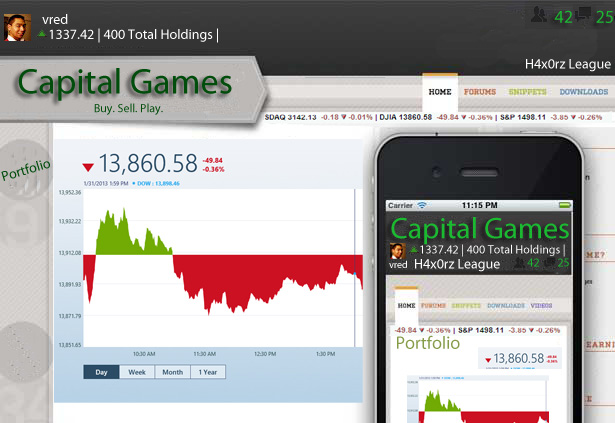
\includegraphics[width=5.5in]{./img/responsiveenough.jpg}

\chapter*{Project Management}
	\addcontentsline{toc}{section}{Project Management}
	
\chapter*{References}
	\addcontentsline{toc}{section}{References}

\end{document}

